\documentclass{article}

\usepackage{amsfonts}
\usepackage{amsmath}
\usepackage{graphicx}
\usepackage{listings}
\lstset{language=R,
		backgroundcolor=\color{black}\ttfamily,
        basicstyle=\color{white}\ttfamily,
        keywordstyle=\color{orange}\ttfamily,
        stringstyle=\color{green}\ttfamily,
        commentstyle=\color{purple}\ttfamily,
        showstringspaces=false
}
\usepackage{xcolor}
\newenvironment{solution}{\color{red}}{\color{black}}

\begin{document}

\title{Recitation 1}
\author{Michael Chirico}

\maketitle

\section{Old-School Probability Basics}

\begin{enumerate}
\item You and a friend each roll a single, unweighted die. What is the probability that your rolls differ by more than two pips?

\begin{solution}
See Figure \ref{fig:dice}. Red regions have differences between rolls of 2 or less; blue are the accepted roll pairs. Since the dice are uniform, simply count blue relative to red squares: $\frac13$.

\begin{figure}[htbp]
\centering
\caption{Joint Distribution of Two Dice Rolls}
\label{fig:dice}
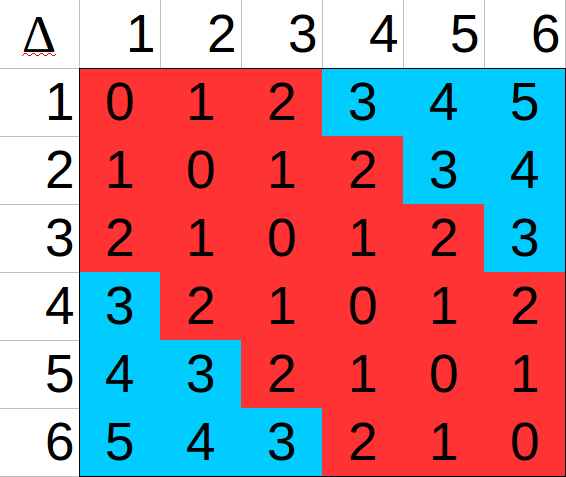
\includegraphics[width = .5\textwidth]{recitation160901_fig1.png}
\end{figure}
\end{solution}

\item Pick a point on the unit square at random (that is, pick two real numbers between 0 and 1 at random). What is the probability they lie in the inscribed circle of the unit square (i.e., the circle which lies inside the square and is tangent to all of its sides)? How could we use this to estimate the value of $\pi$? (Note: while simple, this is a terrible way to estimate $\pi$, and nobody should be estimating $\pi$ anymore anyway. For actual real-world ways to estimate $\pi$ and more discussion, see http://stackoverflow.com/questions/19/ and send your thanks to Ramanujan.)

\begin{solution}
See Figure \ref{fig:circle}. If we pick points at random, the percentage successes is the same as the ratio of the green area to the area of the square, which is $\frac{\pi}4$.

To simulate $\pi$, then, we could check, say, 1,000,000 draws of points in the unit square lie within the green circle. Call the percentage of successes $\hat{p}$. Then we can approximate $\pi$ as $\pi \approx 4\hat{p}$

We could do this in R, for example, as follows:

\begin{lstlisting}
#setting the seed guarantees we'll get
#  exactly the same answer
set.seed(10239)

#draw 1,000,000 x coordinates ~ U[0,1]
draw1 <- runif(1e6)
#draw 1,000,000 y coordinates ~ U[0,1]
draw2 <- runif(1e6)

#count the percentage of successes
success <- (draw1 - .5)^2 + (draw2 - .5)^2 < .5^2
pi_approx <- 4 * mean(success)

pi_approx
# [1] 3.14132
# Not bad!
\end{lstlisting}

\begin{figure}[htbp]
\centering
\caption{Darts in the Unit Square}
\label{fig:circle}
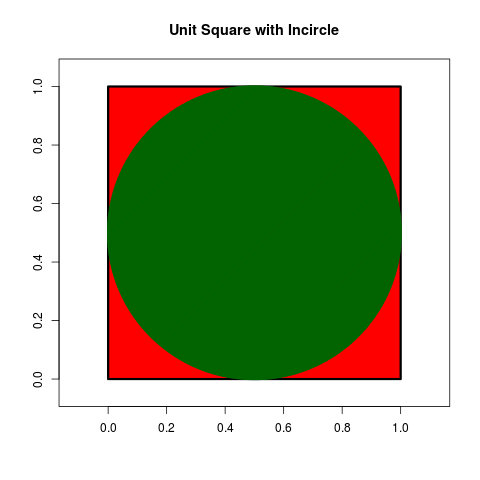
\includegraphics[width = .5\textwidth]{recitation160901_fig2.png}
\end{figure}

Note: I also made the circle-in-square plot in R. Here's that code:

\begin{lstlisting}
#begin empty plot
plot(NULL, xlim = c(-.05, 1.05), 
     ylim = c(-.05, 1.05), asp = 1,
     xlab = "", ylab = "", 
     main = "Unit Square with Incircle")
#plot unit square. see ?polygon
polygon(c(0, 1, 1, 0), c(0, 0, 1, 1), 
        lwd = 3, col = "red")

#plot circle parametrically
xs <- seq(0, 1, length.out = 1000)
#recall equation of general circle:
#  (x - h)^2 + (y - k)^2 = r^2
#  (from Pythagorean Theorem);
#  simply solve this for y and remember
#  we want both branches of the 
#  square root function.
polygon(c(xs, rev(xs)),
        #first branch
        c(.5 + sqrt(.5^2 - (xs - .5)^2),
          #second branch
          .5 - sqrt(.5^2 - (xs - .5)^2)),
        lwd = 3, density = 45, col = "darkgreen")
\end{lstlisting}

\end{solution}

\item \textit{(amended from earlier year's homework)} Suppose we are playing a lottery in which four different bins contain 10 ping-pong balls -- one for each digit -- and a lottery draw consists of a single ball being taken from each bin.
\begin{enumerate}
\item If the lottery requires matching exactly each of the four bins, how many outcomes are there?

\begin{solution}
10 possible outcomes for each bin, 4 bins, no interdependence whatsover $\Rightarrow 10^4$.
\end{solution}

\item If the lottery requires matching the four balls (irrespective of their origin bin), how many outcomes are there?

\begin{solution}
This is equivalent to drawing four balls \textit{with replacement}, where order doesn't matter. Thus the answer is $\dbinom{10 + 4 - 1}{4} = \dbinom{13}4$.

We can calculate this with R!

\begin{lstlisting}
#read the following code from bottom to top!
#  since that's the order the computations
#  are happening
nrow( #get the number of rows
  unique( #eliminate duplicate draws
    as.data.table( #convert to data.table
                   #  so we can use unique
      t( #unfortunately apply flipped
         #  our data, so we flip again
         #  (t = transpose)
        apply( #apply(x, 1, f) will apply
               #  the function f to each
               #  ROW of x. if we wanted
               #  to apply to COLUMNs,
               #  we'd use apply(x, 2, f)
          #expand.grid gives us all
          #  combinations of the vectors
          #  supplied. expand.grid(0:9, 0:9)
          #  would be 10^2 combinations,
          #  expand.grid(0:9, 0:9, 0:9)
          #  would be 10^3 combinations (3 bins)
          expand.grid(0:9, 0:9, 0:9, 0:9),
          #sort each combination from smallest
          #  to largest digit -- that way
          #  both 0,1,0,0 and 0,0,1,0 are
          #  sorted to 0,0,0,1 and thus
          #  considered the same
          1, sort
          )
        )
      )
    )
  )
# [1] 715
choose(13, 4) #checking that it's correct
# [1] 715
\end{lstlisting}
\end{solution}

\end{enumerate}
Suppose instead that all of the 40 balls are in a single bin.
\begin{enumerate}
\item If the lottery requires matching exactly the sequence of four draws, how many outcomes are there?

\begin{solution}
There are 40 balls, and we pick 4 of them \textit{in order}. There are 40 possibilities for the first ball, 39 for the second, 38 for the third, and 37 for the fourth, for a total of $40\cdot 39\cdot 38\cdot 37$ total outcomes. 
\end{solution}

\item If the lottery requires matching the four balls (irrespective of their sequence), how many outcomes are there?

\begin{solution}
There are 40 balls, and we \textit{choose} 4 of them -- and order doesn't matter. Thus there are $\dbinom{40}4$ outcomes.
\end{solution}

\end{enumerate}
\end{enumerate}

\section{Pass the Pigs}

Pass the pigs is a silly dice-like game now produced by Xingcolo, once produced by Milton Bradley:

https://www.amazon.com/exec/obidos/ASIN/B00005JG3Y/probabilitandpig

Players take turns rolling a pair of dice-sized rubber pigs. Depending on how they land, you accumulate points. On each turn, you continue to roll and accumulate points until you choose to pass or until a ``stop'' formation is rolled, at which point your turn ends automatically and you forfeit all points gained on that turn. 

Like a dice, there are six possible outcomes of a roll of a single pig; unlike a dice, the probability of each occurring is not equal.

It's not clear \textit{ex ante} what the exact probability of each outcome actually is; luckily some time-rich fellow named Freddie W. paid some students to conduct an experiment consisting of 3,939 rolls of the pigs (see http://passpigs.tripod.com/prob.html), which gives a sort of empirical distribution of the outcomes, show in Table \ref{tbl:pigout}:

\begin{table}[htbp]
\centering
\begin{tabular}{|r|c|c|}
\hline
Roll Type & Number of Rolls & Proportion \\
\hline
Blank & 1,344 & .341 \\
\hline
Dot & 1,294 & .329 \\
\hline
Razorback & 767 & .195 \\
\hline
Trotter & 365 & .092 \\
\hline
Snouter & 137 & .035 \\
\hline
Leaning Jowler & 32 & .008 \\
\hline
\end{tabular}
\caption{Empirical Likelihood of Pig Roll Types}
\label{tbl:pigout}
\end{table}

\begin{enumerate}
\item What is the probability of rolling a single razorback? (Recall that a roll consists of rolling two pigs at once)

\begin{solution}
Rolling a \textit{single} razorback means rolling one, \textit{but not two} razorbacks. So all told, we want the probability that the first die is a razorback OR the second die is a razorback AND NOT both dice being razorbacks, i.e.,

\[ \mathbb{P}[first\enskip die\enskip razorback] + \mathbb{P}[second\enskip die\enskip razorback] - \mathbb{P}[both\enskip dice\enskip razorback]\]

Which is $.195 + .195 - .195^2$.
\end{solution}

\item What is the probability of rolling a pig-out (one Blank and one Dot)?

\begin{solution}
A pig-out occurs when either the first die is blank and the second is dot, OR the first die is dot and the second is blank. Since the rolls are independent, we simply double the probability of rolling blank AND dot, i.e., $2\cdot .341\cdot .329$.
\end{solution}

\item What is the probability of rolling a double leaning jowler?

\begin{solution}
This means the first die is a leaning jowler AND the second is a leaning jowler. This happens with probability $.008\cdot .008$.
\end{solution}

\item What is the probability of rolling mixed (neither pig is a Dot or a Blank, and the pigs are different)?

\begin{solution}
See Figure \ref{fig:pigs}. Acceptable rolls are (R, T), (R, S), (R, J), (T, S), (T, J), and (S, J), and the reverse. Simply multiply the row probability by the column probability for each of the green squares, and add. To save some time, we only need to do so for the upper triangle (or the lower triangle), then double the result.

\begin{figure}[htbp]
\centering
\caption{Joint Distribution of Pig Tosses}
\label{fig:pigs}
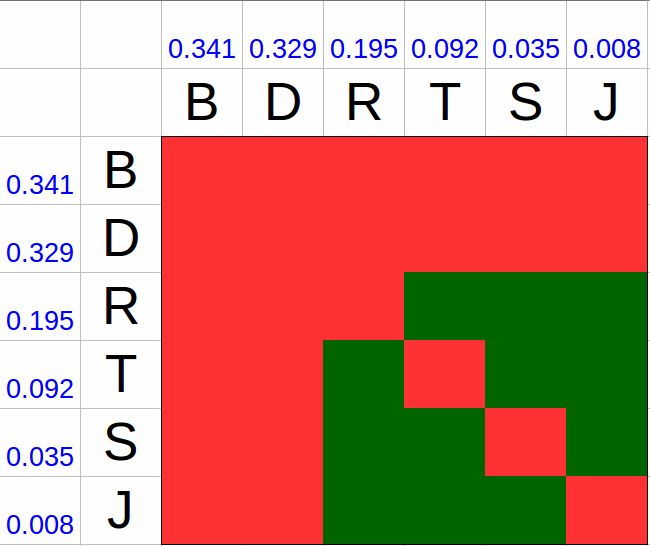
\includegraphics[width = .5\textwidth]{recitation160901_fig3.png}
\end{figure}

\end{solution}

\end{enumerate}

\section{Refugee Screening}

There are about 7 billion people in the world. About 23 million of them live in Syria.

Let's say there are 200,000 terrorists in the world, 30,000 of whom are in Syria.

\begin{enumerate}
\item Given these rough estimates, what is the probability that a randomly selected person in the world is a terrorist?

\begin{solution}
$\frac{200000}{7000000000}$
\end{solution}

\item Given that someone is a terrorist, what is the probability that they are Syrian?

\begin{solution}
See Figure \ref{fig:venn}. ``Given that someone is a terrorist'' means we're ONLY focused on the left-hand circle. Within that circle, 30,000 of the 200,000 total present are terrorists, i.e., $\frac{30000}{200000}$.

\begin{figure}[htbp]
\centering
\caption{Syrian-Terrorist Venn Diagram}
\label{fig:venn}
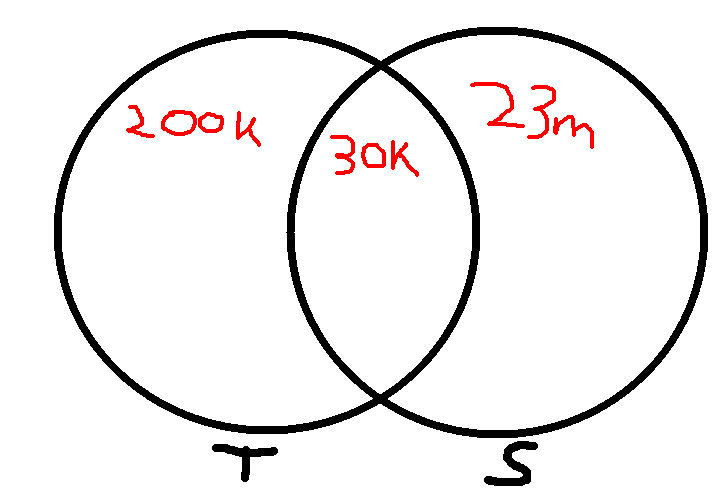
\includegraphics[width = .5\textwidth]{recitation160901_fig4.png}
\end{figure}
\end{solution}

\item You're screening refugees and hoping to weed out any terrorist posing as a refugee. Given that you know the refugee is Syrian, what is the probability they are a terrorist? That is, what is $\mathbb{P}[terrorist|Syrian]$?

\begin{solution}
Using Bayes' rule, we can write

\[ \mathbb{P}[T | S] = \mathbb{P}[S | T] \frac{\mathbb{P}[T]}{\mathbb{P}[S]} = \frac{30000}{200000} \frac{\frac{200000}{7000000000}}{\frac{23000000}{7000000000}} \]
\end{solution}

\item By what order of magnitude does knowing a person is Syrian increase the likelihood that they're a terrorist?

\begin{solution}
This is just $\frac{\mathbb{P}[T | S]}{\mathbb{P}[T]} = \frac{\frac{30000}{200000}}{\frac{23000000}{7000000000}} \approx 45$
\end{solution}

\item \textit{(open-ended/framing thoughts moving forward)} This is of course a simplistic interpretation of the problem of refugee screening. Why does the simplistic analysis break down? What are other important considerations? What assumptions are violated?
\end{enumerate}

\end{document}